This chapter reports the results for the recycle fuel cycle 
scenarios (Scenarios 14-19) described 
in Section \ref{sec:recycle-methods}. The primary results considered 
for these fuel cycle transitions are the uranium resources needed, 
the \gls{SWU} capacity requried, the separated plutonium masses, 
and the mass of material disposed of. This chapter does not focus 
as much on the number of reactors or the energy supplied by 
the reactors because most of the scenarios use the same 
deployment scheme as Scenarios 7 or 14 (depending on 
the energy demand curve of the scenario). For the two 
scenarios that deploy the \gls{SFR} instead of the other 
advanced reactors (Scenarios 16 and 19), the maximum number 
of \glspl{SFR} deployed in each scenario is 312 and 595, 
respectively. 
These scenarios require far fewer reactors than the other scenarios 
because the \gls{SFR} has a larger power output than the other 
advanced reactors (311 MWe compared with 80 MWe for the Xe-100).

\section{Uranium resources}
The uranium resources described here are divided into two primary 
components: the heavy metal mass and the natural uranium 
required to produce fuel. The heavy metal mass is further 
broken into two parts: the mass of enriched uranium and the 
mass of heavy metals in plutonium-based fuel. Enriched uranium 
is in the 
\gls{HALEU}, \gls{UOX}, and UCO fuels. Heavy metals in plutonium-based 
fuels include the natural uranium, plutonium, and transuranics in 
the \gls{MOX} and U/TRU fuels. The separation of these metrics 
stems from the different processes and resources needed to 
produce each fuel type. The natural uranium masses are also 
broken into two parts: feed uranium to produce enriched uranium 
and the mass of natural uranium required to produce 
plutonium-based fuel (\gls{MOX} or U/TRU fuel). This separation 
of this metric provides more detailed insights into for 
what the resources are needed as well as how much are needed. 

\subsection{No growth scenarios}
\subsubsection{Fuel masses}
The mass of enriched uranium required by the no growth 
closed fuel cycles are shown in Figure \ref{fig:nogrowth_recycle_uranium}.
Scenario 15 requires the most enriched uranium, followed by 
Scenario 14, then Scenario 16. Scenario 15 requires the most enriched 
uranium because less material is available for reprocessing, leading to 
less separated plutonium available to produce \gls{MOX} fuel.

\begin{figure}[h!]
    \centering
    \begin{subfigure}[b]{0.45\textwidth}
        \centering
        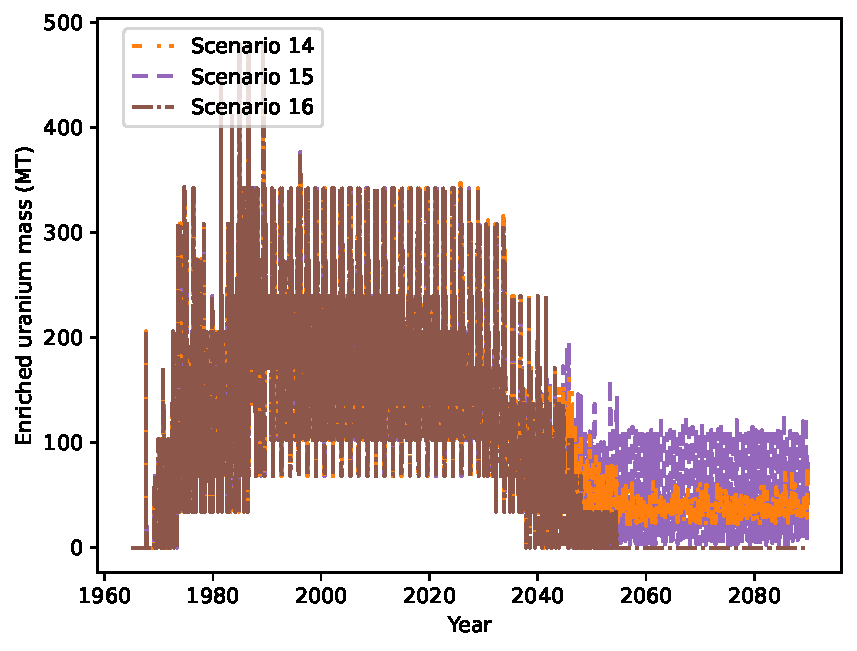
\includegraphics[width=\textwidth]{nogrowth_recycle_total_fuel.pdf}
        \caption{Monthly mass of enriched uranium sent to all reactors 
        between 1965-2090.}
        \label{fig:nogrowth_recycle_all_uranium}
    \end{subfigure}
    \hfill
    \begin{subfigure}[b]{0.45\textwidth}
        \centering
        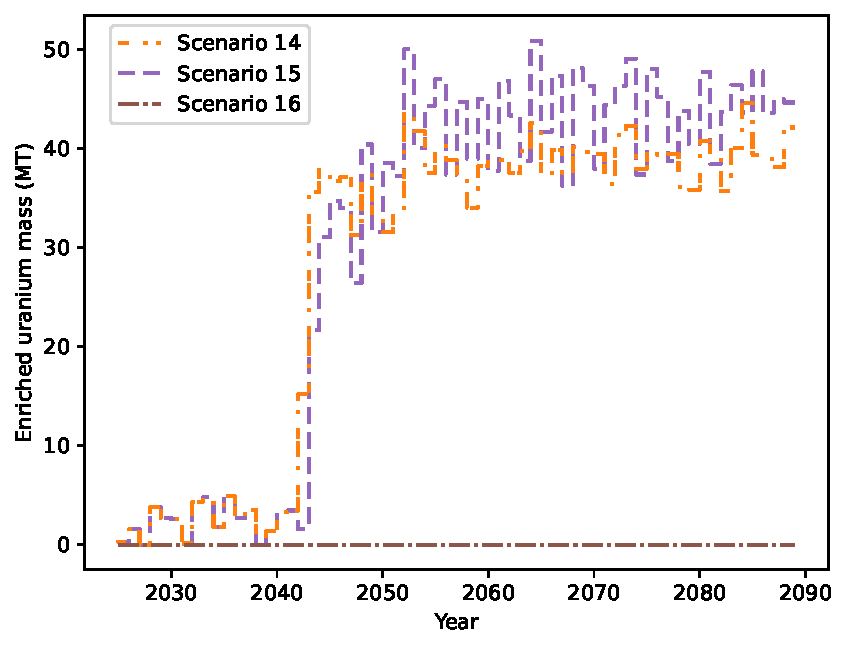
\includegraphics[width=\textwidth]{nogrowth_recycle_Uaverages.pdf}
        \caption{Annual average mass of enriched uranium sent to 
        advanced reactors between 2025-2090.}
        \label{fig:nogrowth_recycle_AR_uranium}
    \end{subfigure}
    \begin{subfigure}[b]{0.45\textwidth}
        \centering
        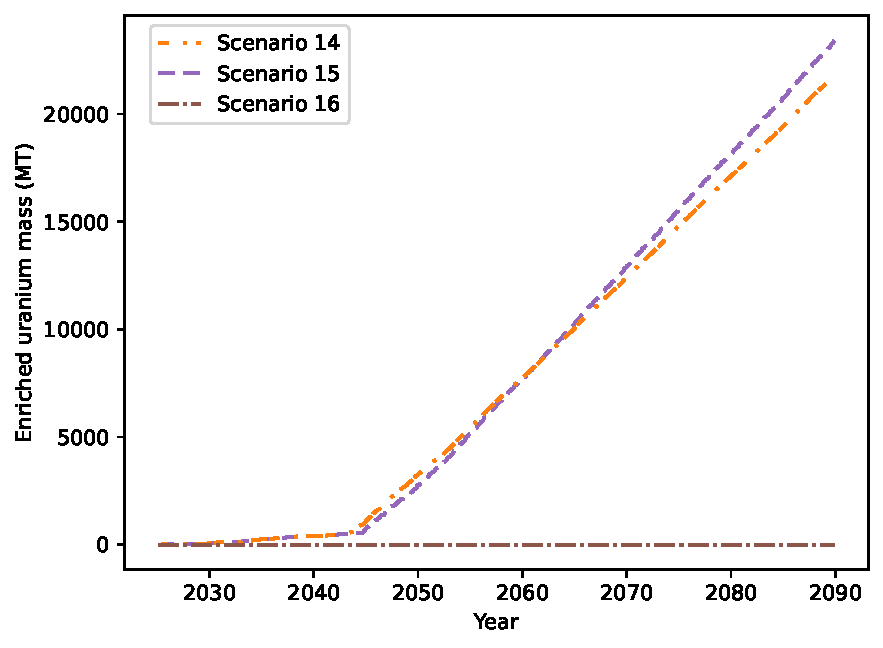
\includegraphics[width=\textwidth]{nogrowth_recycle_Ucumulative.pdf}
        \caption{Cumulative mass of enriched 
        uranium sent to advanced reactors between 2025-2090.}
        \label{fig:nogrowth_recycle_uranium_cumulative}
    \end{subfigure}
       \caption{Mass of enriched uranium required by reactors
        in Scenarios 14-16.}
       \label{fig:nogrowth_recycle_uranium}
\end{figure}

The annual average mass of enriched uranium in Scenarios 14 and 15 increases 
in 2043 because the \gls{MOX} stockpiled up from the \gls{LWR} \gls{SNF} 
is used up and there is not as much plutonium from the advanced reactor 
\gls{SNF} to produce more \gls{MOX} fuel. 

Table \ref{tab:s14-16_uranium} reports the average enriched uranium mass, 
average \gls{HALEU} mass, maximum enriched uranium mass, and cumulative 
enriched uranium mass required by these scenarios. Scenario 14 requires 
less enriched uranium than Scenario 7, despite having the same 
advanced reactor deployment schedule, because of the change in the 
fuel cycle. By reprocessing spent fuel, the average \gls{HALEU} 
mass required drops by 21.3\%. However, the metrics of Scenario 15 
highlight how the types of materials available for reprocessing 
affects the impact of the fuel cycle option. 

\begin{table}[h!]
    \centering 
    \caption{Metrics for enriched uranium required to fuel reactors 
    in Scenarios 14-16.}
    \label{tab:s14-16_uranium}
    \begin{tabular}{c c c c c}
        \hline 
        Scenario & Average (MT/month) & HALEU Average (MT/month) 
        & Maximum (MT) & Cumulative (MT) \\
        \hline 
        14 & 28.01 & 27.16 & 87.01 & 21,920 \\
        15 & & & & \\
        16 & 0 & 0 & 0 & 0\\
        \hline
        
    \end{tabular}
\end{table}

Scenario 16 does not require any uranium-based fuel to support the 
advanced reactors. This result stems from a few key differences between 
these fuel cycles. The first difference is that all of the advanced 
reactors in Scenario 16 can accept reprocessed fuel, while the \glspl{MMR} 
in Scenarios 14 and 15 will only accept \gls{UOX}. This modeling 
decision for the \gls{MMR} means that any fuel cycle that 
deploys the \gls{MMR} will always require some amount of uranium-based 
fuel. The second is amount of times the fuel can be reprocessed. 
In Scenario 16, the spent fuel can be reprocessed an infinite number 
of times and in Scenarios 14 and 15 the spent uranium-based fuel can 
only be reprocessed once and the plutonium-based fuel can not be 
reprocessed. This difference is inherent to the type of fuel cycle 
(limited vs. continuous recycle) and is the primary driver of the 
why Scenario 16 does not require any uranium-base fuels for the 
advanced reactors. 

The advanced reactors in Scenario 16 do not require any uranium-based fuel, 
so they are all supplied plutonium-based fuels. Figure 
\ref{fig:nogrowth_recycle_mox} shows that Scenario 16 requires more 
plutonium-based fuel than the other scenarios. As Table 
\ref{tab:s14-16_mox} reports, Scenario 16 needs a monthly average 
of plutonium-based fuel that is larger than the maximum mass 
needed in Scenarios 14 and 15. 

\begin{figure}[h!]
    \centering
    \begin{subfigure}[b]{0.45\textwidth}
        \centering
        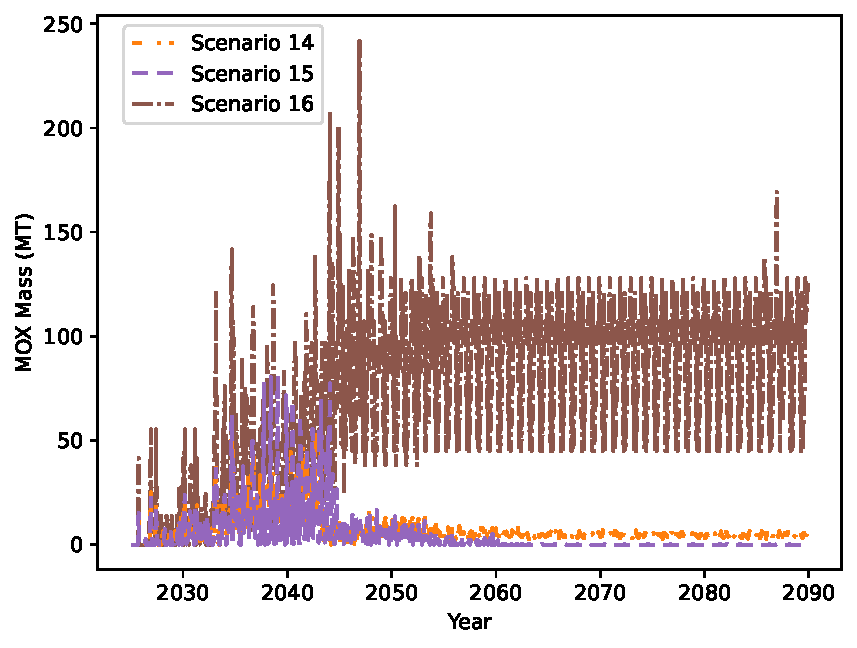
\includegraphics[width=\textwidth]{nogrowth_recycle_MOX.pdf}
        \caption{Monthly masses of plutonium-based fuel sent to 
        advanced reactors between 2025-2090.}
        \label{fig:nogrowth_recycle_AR_mox}
    \end{subfigure}
    \hfill
    \begin{subfigure}[b]{0.45\textwidth}
        \centering
        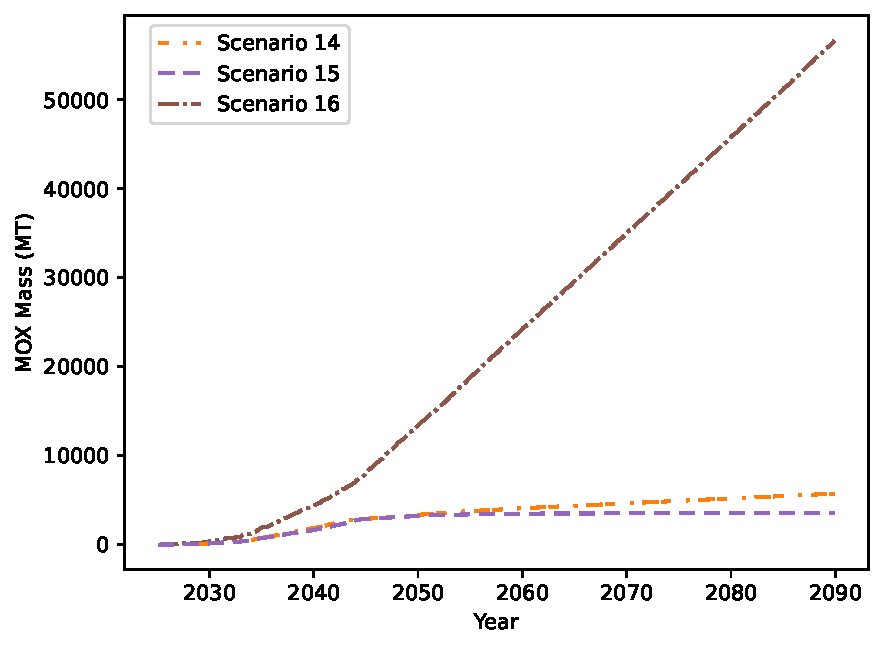
\includegraphics[width=\textwidth]{nogrowth_recycle_MOXcumulative.pdf}
        \caption{Cumulative mass of plutonium-based fuel
        sent to advanced reactors between 2025-2090.}
        \label{fig:nogrowth_recycle_mox_cumulative}
    \end{subfigure}
       \caption{Mass of plutonium-based fuel required by reactors
        in Scenarios 14-16.}
       \label{fig:nogrowth_recycle_mox}
\end{figure}

\begin{table}[h!]
    \centering 
    \caption{Metrics for plutonium-based fuels required to fuel reactors 
    in Scenarios 14-16.}
    \label{tab:s14-16_mox}
    \begin{tabular}{c c c c}
        \hline 
        Scenario & Average (MT/month) & Maximum (MT) & Cumulative (MT) \\
        \hline 
        14 & 7.351 & 53.81 & 5,727 \\
        15 & & &  \\
        16 & 72.70 & 241.9 & 56,630 \\
        \hline
        
    \end{tabular}
\end{table}

When comparing the total cumulative mass of heavy metal (enriched 
uranium and heavy metal in plutonium-based fuel) required by each scenario,
Scenario 16 needs the most material to support the advanced reactors. This 
result stems from the different discharge burnups of the reactors. The 
\gls{SFR} has a burnup of 87.51 MWd/kg HM and the Xe-100 (the reactor that 
meets most of the demand in Scenarios 14 and 15) has a burnup of 168 MWd/kg U. 
The Xe-100 gets more energy out of each unit mass of fuel, which leads to 
Scenarios 14 and 15 requiring less fuel than Scenario 16. Scenario 16 is most 
similar to Scenario 2 in the amount of heavy metals required. This result 
stems from the \gls{SFR} and \gls{MMR} having similar discharge burnups.

\subsubsection{Natural uranium}
The natural uranium required as feed uranium to produce enriched 
uranium fuel for reactors is shown in Figure \ref{fig:nogrowth_recycle_feed}.


\begin{figure}[h!]
    \centering
    \begin{subfigure}[b]{0.45\textwidth}
        \centering
        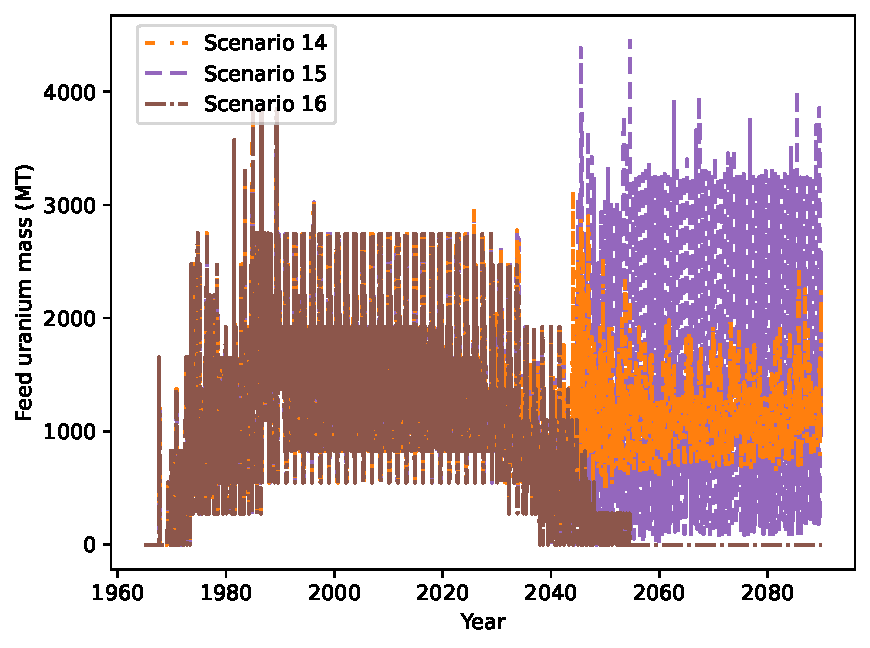
\includegraphics[width=\textwidth]{nogrowth_recycle_feed.pdf}
        \caption{Monthly mass of enriched uranium sent to all reactors 
        between 1965-2090.}
        \label{fig:nogrowth_recycle_all_feed}
    \end{subfigure}
    \hfill
    \begin{subfigure}[b]{0.45\textwidth}
        \centering
        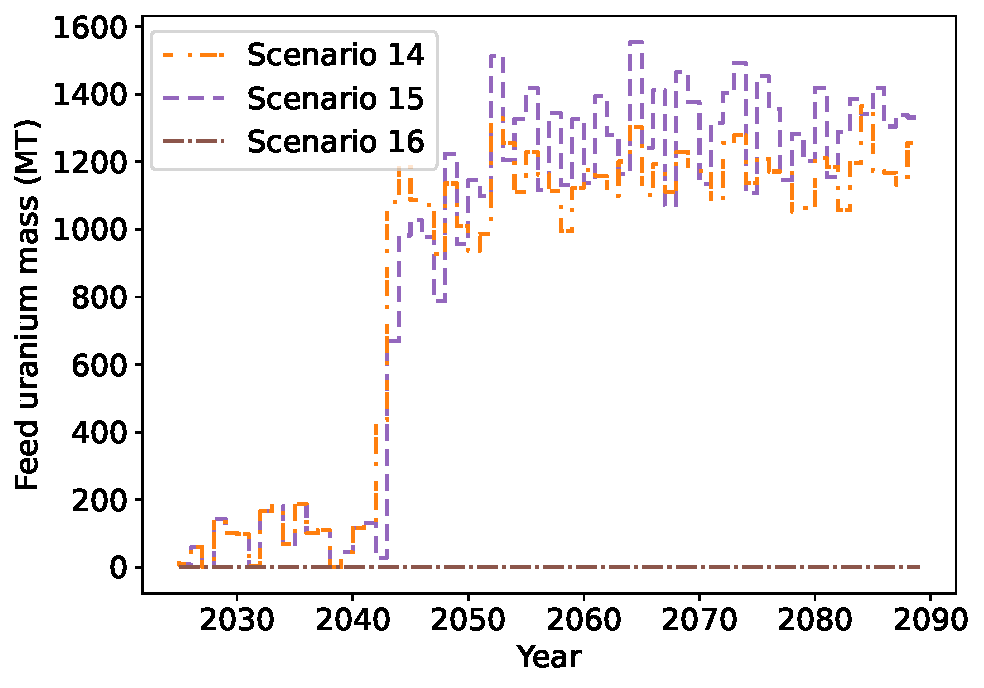
\includegraphics[width=\textwidth]{nogrowth_recycle_feed_average.pdf}
        \caption{Annual average mass of enriched uranium sent to 
        advanced reactors between 2025-2090.}
        \label{fig:nogrowth_recycle_AR_feed}
    \end{subfigure}
    \begin{subfigure}[b]{0.45\textwidth}
        \centering
        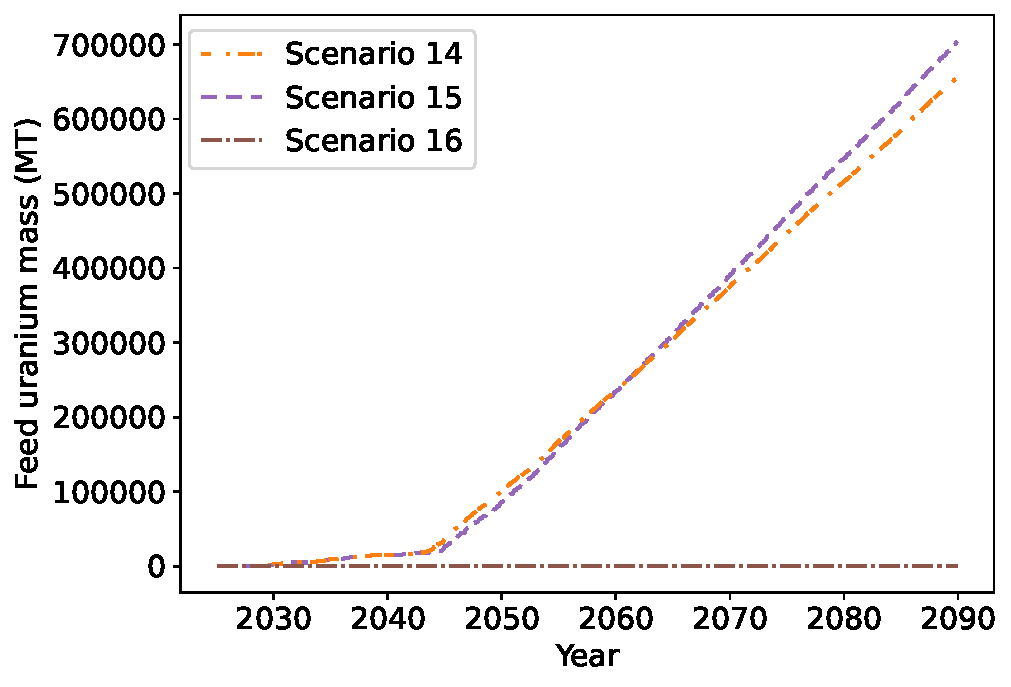
\includegraphics[width=\textwidth]{nogrowth_recycle_feed_cumulative.pdf}
        \caption{Cumulative mass of enriched 
        uranium sent to advanced reactors between 2025-2090.}
        \label{fig:nogrowth_recycle_feed_cumulative}
    \end{subfigure}
       \caption{Mass of enriched uranium required by reactors
        in Scenarios 14-16.}
       \label{fig:nogrowth_recycle_feed}
\end{figure}

\begin{table}[h!]
    \centering 
    \caption{Metrics for feed uranium required to produce 
    uranium-based fuels in in Scenarios 14-16.}
    \label{tab:s14-16_feed}
    \begin{tabular}{c c c c c}
        \hline 
        Scenario & Average (MT/month) & HALEU Average (MT/month) &
        Maximum (MT) & Cumulative (MT) \\
        \hline 
        14 & 842.9 & 836.4 & 2,628 & 656,582 \\
        15 & & & & \\
        16 & 0 & 0 & 0 & 0\\
        \hline
        
    \end{tabular}
\end{table}



\begin{figure}[h!]
    \centering
    \begin{subfigure}[b]{0.45\textwidth}
        \centering
        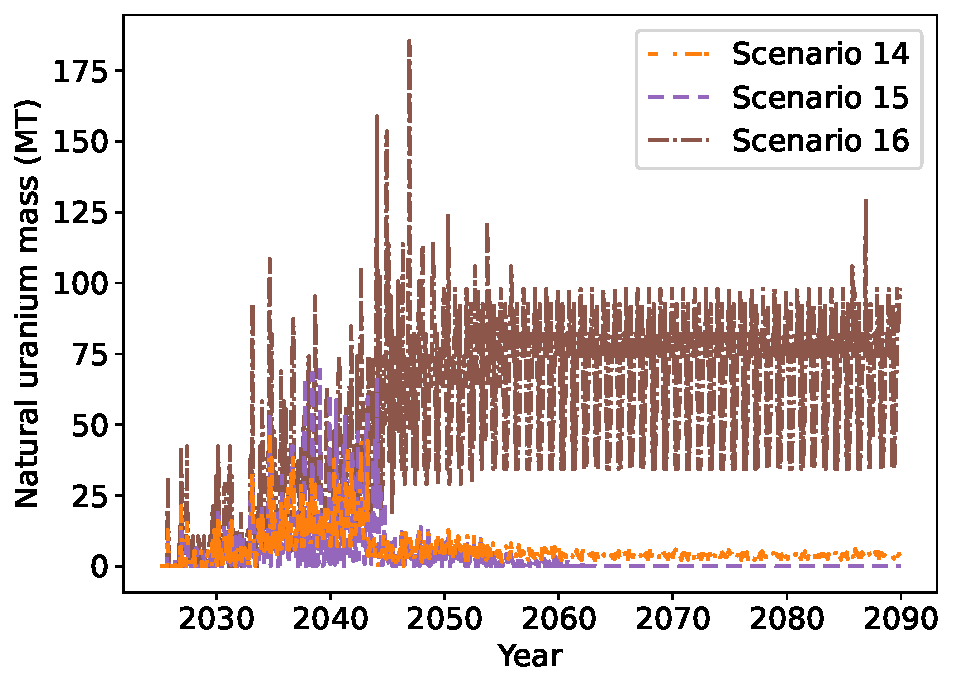
\includegraphics[width=\textwidth]{nogrowth_recycle_natU.pdf}
        \caption{Monthly masses of plutonium-based fuel sent to 
        advanced reactors between 2025-2090.}
        \label{fig:nogrowth_recycle_AR_natu}
    \end{subfigure}
    \hfill
    \begin{subfigure}[b]{0.45\textwidth}
        \centering
        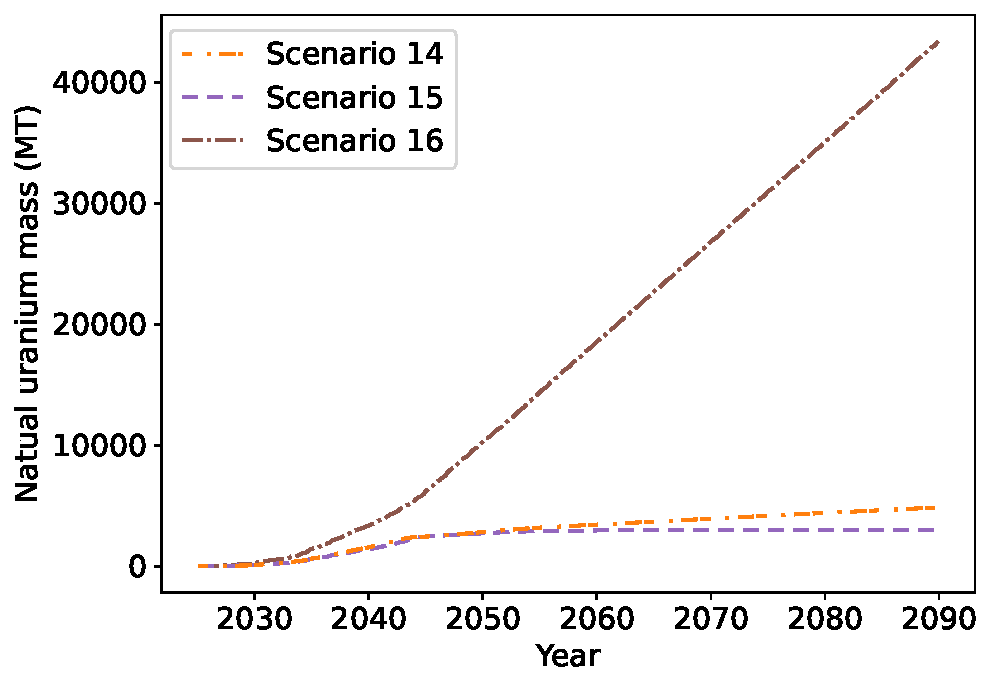
\includegraphics[width=\textwidth]{nogrowth_recycle_natU_cumulative.pdf}
        \caption{Cumulative mass of plutonium-based fuel
        sent to advanced reactors between 2025-2090.}
        \label{fig:nogrowth_recycle_natu_cumulative}
    \end{subfigure}
       \caption{Mass of plutonium-based fuel required by reactors
        in Scenarios 14-16.}
       \label{fig:nogrowth_recycle_natu}
\end{figure}

\begin{table}[h!]
    \centering 
    \caption{Metrics for natural uranium required to produce 
    plutonium-based fuels in Scenarios 14-16.}
    \label{tab:s14-16_natU}
    \begin{tabular}{c c c c}
        \hline 
        Scenario & Average (MT/month) & Maximum (MT) & Cumulative (MT) \\
        \hline 
        14 & 6.256 & 45.80 & 4,874 \\
        15 & & &  \\
        16 & 55.68 & 185.3 & 43,372 \\
        \hline
        
    \end{tabular}
\end{table}



\subsection{1\% growth scenarios}

\section{SWU capacity}
\subsection{No growth scenarios}

\begin{figure}[h!]
    \centering
    \begin{subfigure}[b]{0.45\textwidth}
        \centering
        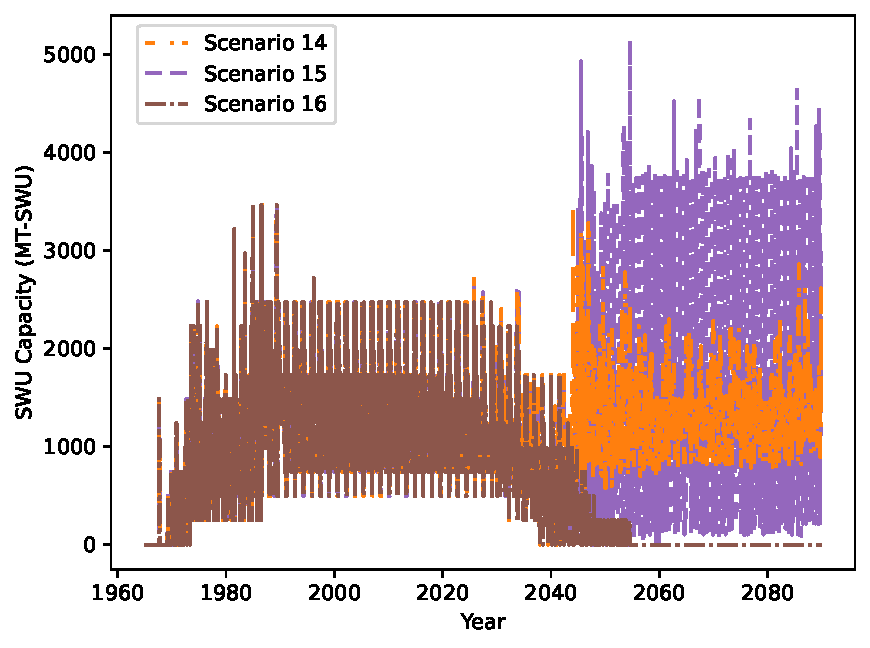
\includegraphics[width=\textwidth]{nogrowth_recycle_swu.pdf}
        \caption{Monthly SWU capacity required to produce 
        enriched uranium for all reactors between 2025-2090.}
        \label{fig:nogrowth_recycle_swu_all}
    \end{subfigure}
    \hfill
    \begin{subfigure}[b]{0.45\textwidth}
        \centering
        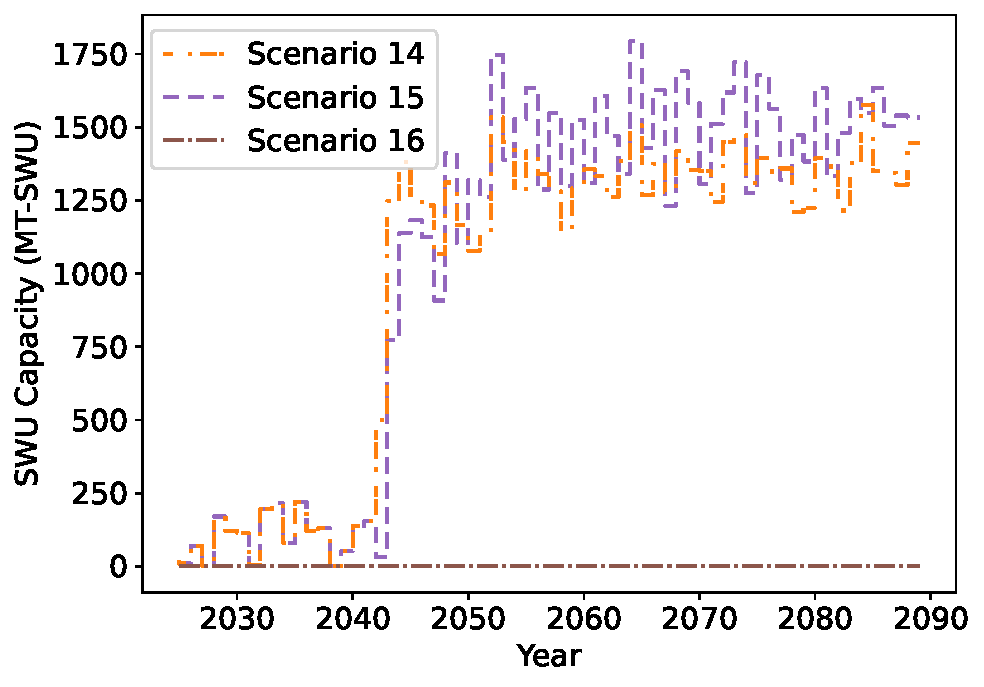
\includegraphics[width=\textwidth]{nogrowth_recycle_AR_swu.pdf}
        \caption{Monthly SWU capacity required to produce 
        enriched uranium for advanced reactors between 2025-2090.}
        \label{fig:nogrowth_recycle_swu_AR}
    \end{subfigure}
       \caption{\gls{SWU} capacity required in Scenarios 14-16.}
       \label{fig:nogrowth_recycle_swu}
\end{figure}

\begin{table}[h!]
    \centering 
    \caption{Metrics for \gls{SWU} capacity required to produce 
    enriched uranium in Scenarios 14-16.}
    \label{tab:s14-16_swu}
    \begin{tabular}{c c c c}
        \hline 
        Scenario & Average (MT-SWU/month) & HALEU Average (MT-SWU/month)
         & Maximum (MT-SWU) \\
        \hline 
        14 & 971.6 & 965.9 & 3,032 \\
        15 & & &  \\
        16 & 0 & 0 & 0 \\
        \hline
        
    \end{tabular}
\end{table}

\subsection{1\% growth scenarios}

\section{Separated plutonium}
The separated plutonium mass reported is the material mass traded 
between the separations and fuel fabrication facility in each 
scenario. 

\subsection{No growth scenarios}

\subsection{1\% growth scenarios}

\section{Spent nuclear fuel and High Level Waste}
This section provides the results of the \gls{SNF} and \gls{HLW} sent 
to disposal in the closed fuel cycles. The once-through scenario 
results only defined the \gls{SNF} sent for disposal because all 
of the materials needing disposal in those scenarios are \gls{SNF}. 
With the addition of the separation step, the \gls{SNF} discharged 
from reactors gets separated into two different material streams, 
one of the separated plutonium and one of \gls{HLW} that is sent 
for disposal.

\subsection{No growth scenarios}
This section presents the results of the \gls{SNF} and 
\gls{HLW} masses that are sent for disposal in a 
material sink in the no growth recycle scenarios. 
\subsubsection{Spent nuclear fuel}

\subsubsection{High level waste}


\subsection{1\% growth scenarios}
This section presents the results of the \gls{SNF} and 
\gls{HLW} masses that are sent for disposal in a 
material sink in the 1\% growth recycle scenarios. 
\subsubsection{Spent nuclear fuel}

\subsubsection{High level waste}